\documentclass[tikz,border=4pt]{standalone}
\usepackage{pifont}
\usepackage{tikz}
\usepackage{amsmath}
\usetikzlibrary{calc,arrows.meta,positioning,shapes.geometric}

\begin{document}
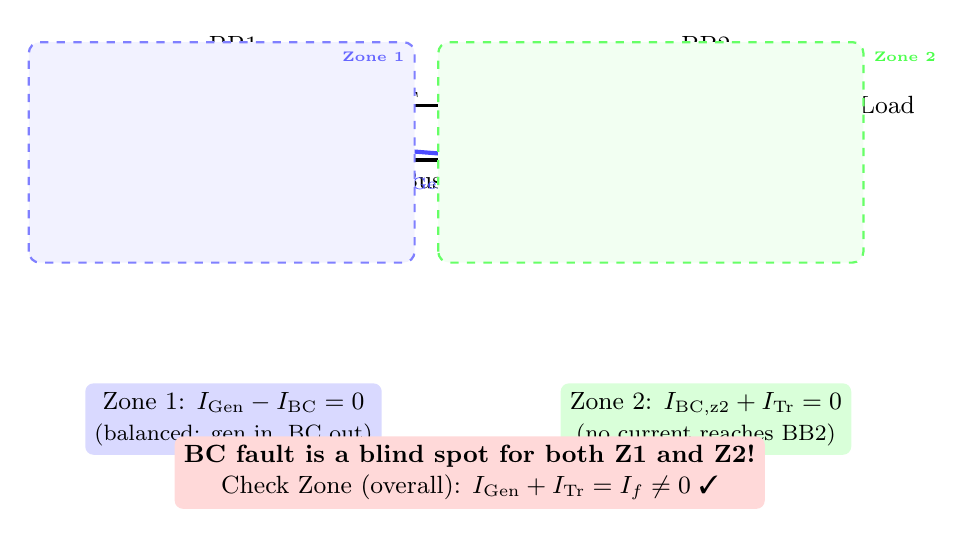
\begin{tikzpicture}[
    bus/.style={draw,fill=gray!25,minimum width=0.4cm,minimum height=2.4cm,
                line width=1.5pt,inner sep=0pt},
    ct/.style={draw,circle,fill=white,inner sep=1.5pt,font=\small,
               minimum size=0.5cm,line width=0.8pt},
    fault/.style={draw,fill=red!70,regular polygon,regular polygon sides=3,
                  minimum size=0.5cm,font=\footnotesize\bfseries,text=white,
                  inner sep=0pt},
    arr/.style={-{Latex[length=2.5mm]},line width=1.0pt},
    darr/.style={-{Latex[length=2.5mm]},line width=1.0pt,red!70},
    ann/.style={font=\small},
    zone/.style={draw,dashed,rounded corners=4pt,line width=0.8pt},
]

% ---- BB1 and BB2 ---------------------------------------------------------
\node[bus,label={[font=\small]above:BB1}] (bb1) at (0,0) {};
\node[bus,label={[font=\small]above:BB2}] (bb2) at (6,0) {};

% ---- Gen feeder ----------------------------------------------------------
\node[ann] (gen) at (-2.2, 0.7) {Gen};
\draw[arr] (gen.east) -- (-0.2, 0.7);
\node[ct] at (-1.1, 0.7) {CT};

% ---- Transformer feeder --------------------------------------------------
\node[ann] (tr) at (8.3, 0.7) {Load};
\draw[arr] (0.2, 0.7) to[bend right=0] (tr.west);
% CT on transformer feeder
\node[ct] at (7.1, 0.7) {CT};

% ---- Bus coupler ---------------------------------------------------------
\draw[line width=1.5pt] (0.2, 0) -- (5.8, 0)
    node[midway,below,ann] {Bus Coupler};
% BC CT is on BB1-side
\node[ct,fill=yellow!30] (ctBC) at (1.5, 0.2) {CT};
\node[ann,above] at (1.5, 0.55) {\footnotesize BB1-side CT};

% ---- Fault inside BC (between CT and BB2) --------------------------------
\node[fault] (fault) at (3.8, 0) {F};
\node[ann,above=0.15cm of fault] {\footnotesize BC fault};

% ---- Current arrows during BC fault ------------------------------------
% Gen current flows: Gen → BB1 → BC → CT → Fault
\draw[darr,blue!70,line width=1.5pt]
    (-2.0,0.3) -- (-0.1,0.3) -- (-0.1,-0.05)
    -- (ctBC.west|-{(0,-0.05)}) -- (ctBC.west)
    -- (3.7, 0)
    node[midway,below=2pt,ann,text=blue!70] {$I_{\rm Gen}$};

% ---- Zone 1 boundary (Gen CT + Line CT + BC CT) -------------------------
\draw[zone,blue!50,fill=blue!5]
    (-2.6,-1.3) rectangle (2.3, 1.5)
    node[below left, font=\tiny\bfseries, text=blue!60] {Zone 1};

% ---- Zone 2 boundary (BC other side + TR CT) ----------------------------
\draw[zone,green!60,fill=green!5]
    (2.6,-1.3) rectangle (8.0, 1.5)
    node[below right, font=\tiny\bfseries, text=green!70] {Zone 2};

% ---- Differential annotations -------------------------------------------
\node[fill=blue!15,rounded corners=3pt,font=\small,align=center,
      below=1.6cm of bb1]
    {Zone 1: $I_{\rm Gen} - I_{\rm BC} = 0$\\
     \footnotesize(balanced: gen in, BC out)};

\node[fill=green!15,rounded corners=3pt,font=\small,align=center,
      below=1.6cm of bb2]
    {Zone 2: $I_{\rm BC,z2} + I_{\rm Tr} = 0$\\
     \footnotesize(no current reaches BB2)};

\node[fill=red!15,rounded corners=3pt,font=\small,align=center,
      below=3.5cm of {(3,0)}]
    {\textbf{BC fault is a blind spot for both Z1 and Z2!}\\
     Check Zone (overall): $I_{\rm Gen} + I_{\rm Tr} = I_f \neq 0$ \ding{51}};

\end{tikzpicture}
\end{document}
